\documentclass{bmvc2k}
\usepackage[utf8]{inputenc}
%% Enter your paper number here for the review copy
% \bmvcreviewcopy{??}

\usepackage{dirtytalk}
\usepackage{float}

\renewcommand{\figurename}{Figura}
\renewcommand{\refname}{Referencias}

\title{Memoria visual de un robot usando redes neuronales}

% Enter the paper's authors in order
% \addauthor{Name}{email/homepage}{INSTITUTION_CODE}
\addauthor{Alexandre Rodríguez Rendo Estudiante}{http://jderobot.org/Arodriguez-tfm}{1}

% Enter the institutions
% \addinstitution{Name\\Address}
\addinstitution{
 Máster Oficial en Visión Artificial\\
 Universidad Rey Juan Carlos\\
 Móstoles, España
}


\runninghead{Introducción a la Investigación}{Trabajo sobre el Estado del Arte}

% Any macro definitions you would like to include
% These are not defined in the style file, because they don't begin
% with \bmva, so they might conflict with the user's own macros.
% The \bmvaOneDot macro adds a full stop unless there is one in the
% text already.
\def\eg{\emph{e.g}\bmvaOneDot}
\def\Eg{\emph{E.g}\bmvaOneDot}
\def\etal{\emph{et al}\bmvaOneDot}

%-------------------------------------------------------------------------
% Document starts here
\begin{document}

\maketitle

\begin{abstract}
Este documento trata de cubrir todos los requisitos necesarios a la hora
de redactar un artículo sobre el Estado del Arte de un determinado tema.
En este caso, se pretende que este trabajo sea la base empleada para las secciones
de Introducción y Estado del Arte típicas del Trabajo de Fin de Máster.
En dicho trabajo se tratará de crear una memoria visual en un robot empleando técnicas de tracking, segmentación y clasificación,
principalmente, con la ayuda de redes neuronales.
\end{abstract}

%-------------------------------------------------------------------------
\section{Introducción}
\label{sec:intro}
El objetivo general de este trabajo se centra en implementar una memoria visual en un robot
utilizando redes neuronales y una técnica novedosa para segmentación semántica de imágenes, \textit{Mask R-CNN}. Para ello se hará uso de una de las plataformas existentes para el desarrollo de dichas redes, Keras. Esta memoria visual tiene como objetivo enseñar al robot a "entender" el entorno. En este entorno deberá ser capaz de diferenciar clases como humanos, puertas o mesas.\\

En esta sección se situará el trabajo en el marco actual, comenzando por explicar de forma genérica en qué consisten la Robótica y la Visión Artificial. Tras ello, se realizará una introducción a las redes neuronales y algunos de los entornos de Deep Learning. Por último, se expondrán los objetivos concretos de este proyecto definidos hasta el momento.

\subsection{Robótica y Visión Artificial}
Los campos de la Robótica y la Visión Artificial se encuentran íntimamente relacionados en la actualidad y afrontan los retos del desarrollo de las capacidades básicas requeridas por sistemas semi-autónomos y autónomos para ejecutar tareas complejas en el mundo real. Así, la tendencia indica que deberán seguir un camino paralelo para resolver los problemas futuros que van a surgir. Algunas de estas capacidades requeridas son el procesamiento e interpretación de los datos del sensor o sensores, la construcción de modelos espacio-temporales del mundo exterior y el razonamiento sobre ellos, la auto-localización o las interfaces entre humano y máquina [1]. Cuando se utilizan robots cuyos sensores principales son cámaras, como el proyecto que se trata, la interpretación que el robot hace de los datos obtenidos no es tan inmediata como puede ser la obtenida con otros sensores como laser. Aquí es donde entra en juego la importancia de la visión artificial en robótica.

Una de las áreas donde más se están utilizando los robots es la industria. Esta se ha caracterizado por su constante cambio y en la actualidad nos encontramos en la cuarta revolución industrial, más conocida como Industria 4.0. Se basa en sistemas de producción cibernéticos y automatizados, utilizando grandes volúmenes de datos y tecnologías para la manufactura. Con ella los robots han ido evolucionando desde la automatización de determinados procesos industriales hasta la actualidad, donde se buscan sistemas robóticos inteligentes y perceptivos [2].\\
Los sistemas que utilizan Visión Artificial en la industria se conocen como sistemas de visión o visión por máquina (\textit{Machine vision}) y son ampliamente empleados. Sus propósitos principales son los procesos de inspección y control de calidad (Figura \ref{fig:robot}), donde a través de una serie de medidas en las características, componentes u otros parámetros de un producto se verifica si cumple con los requisitos especificados. Pero existen muchas otras aplicaciones como la manufactura de componentes electrónicos, la biometría o los sistemas de seguridad en entornos industriales [3]. También cabe mencionar la importancia de los sistemas de visión en el movimiento del robot y el posicionamiento preciso. Este es un aspecto crucial en muchas de las operaciones que realizan los robots en áreas como la automoción o la industria aeroespacial. Así en los procesos se requiere de una precisión y un margen de error en el movimiento que varía en cada una de las áreas. Por ello, la combinación con métodos de calibrado óptico que pueden ofrecer los sistemas de visión es de gran importancia.
\begin{figure}[H]
\begin{center}
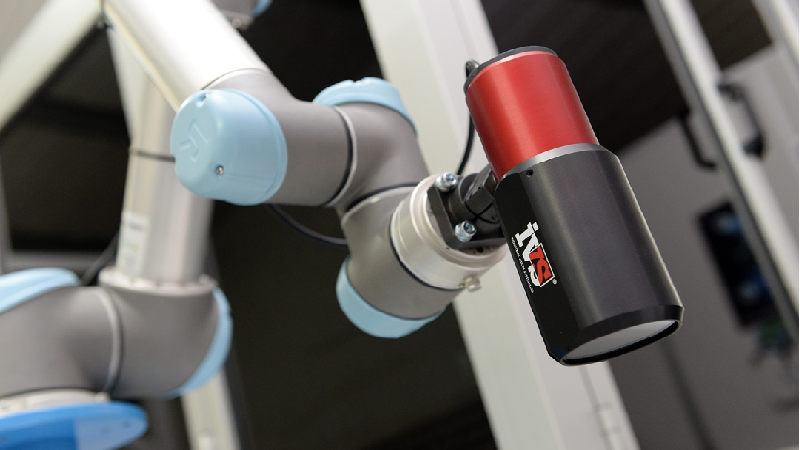
\includegraphics[scale=0.3]{Collaborative-Robot-Inspection.png}
\caption{Inspección robótica}
\label{fig:robot}
\end{center}
\end{figure}
\noindent Otros sectores como el de la logística están siendo transformados a través de robots que se encargan de realizar tareas como el embalaje, transporte o recogida del producto (Figura \ref{fig:logistica}). Con esto se pretende, entre otros motivos, satisfacer la exigencia del cliente en términos de entregas rápidas y eficientes. Además de esto existen numerosas aplicaciones que surgen de la unión de Robótica y Visión Artificial, principalmente, que se están comenzando a utilizar en el día a día. Ejemplo de ello es la irrupción completa del coche autónomo en el panorama automovilístico donde se afrontan problemas que van desde la reconstrucción estéreo, la calibración de las cámaras del vehículo hasta la detección de objetos [3,1]. Por último, es necesario mencionar una de las aplicaciones más conocidas de la robótica, se trata del robot aspiradora al que ya no es novedad encontrar en muchos hogares.
\begin{figure}[h!]
\begin{center}
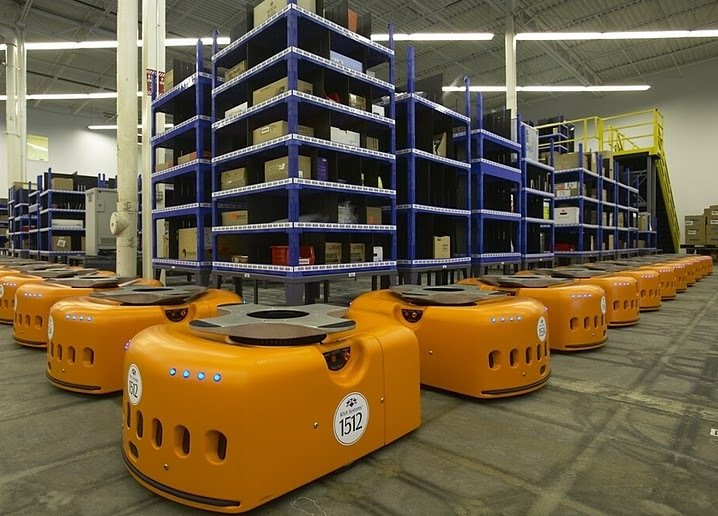
\includegraphics[scale=0.2]{amazonlogistics.jpg}
\caption{Robots en logística de almacenes}
\label{fig:logistica}
\end{center}
\end{figure}

\subsection{Redes Neuronales en Visión Artificial}
Desde el nacimiento de la Inteligencia Artificial (IA) en 1956 [4] la robótica y la visión artificial han seguido un gran ritmo de evolución. Llevando a las máquinas a igualar a los humanos en la resolución de algunas tareas, y en ciertos casos, a superarlos.
La inteligencia artificial se define en [5] como "el subcampo de las Ciencias de la Computación dedicado a desarrollar programas que permitan a los ordenadores presentar comportamientos que se puedan caracterizar como inteligentes". El aprendizaje máquina o \textit{Machine Learning} (\textit{ML}) se define en [6] como "un campo de las Ciencias de la Computación que dá a los ordenadores la capacidad de aprender sin explícitamente programados". Por tanto, dada esta definición, el ML se puede considerar un subcampo de la IA.\\
Uno de los subcampos del ML más conocidos y en auge actualmente es el denominado \textit{Deep Learning}[6,1]. Este tipo de algoritmos se encuentra íntimamente ligado con las Redes Neuronales Artificiales (\textit{ANN}) y en la práctica se suelen usar de forma equivalente aunque no son lo mismo. Uno de los aspectos a destacar en los algoritmos de Deep Learning es que ya no es necesario extraer vectores de características para la entrada a la red. Esto es así porque dichos algoritmos "aprenden" a representar los datos de forma jerárquica. Dentro de estas redes tienen especial interés en la visión artificial y en el problema que afronta este proyecto las redes neuronales convolucionales. Este tipo de redes se caracterizan por utilizar una operación convolución en al menos una de las capas de la red y están diseñadas para el procesado de datos dos-dimensionales como pueden ser las imágenes [6,2]. En los últimos años, su evolución ha sido constante llegando a superar los resultados conseguidos por algoritmos anteriormente en tareas como clasificación o detección de objetos.\\
Para el uso de Deep Learning han surgido numerosos entornos, estos son algunos de los más empleados en la actualidad:
\begin{itemize}
\item \textbf{Tensorflow}: ofrece un API de bajo nivel que permite un control completo sobre los diseños de los modelos y también un API de alto nivel más simplificado pero con una funcionalidad limitada. Además permite la visualización del entrenamiento mediante la herramienta Tensorboard.
\item \textbf{Keras}: proporciona un API de alto nivel para uso de redes de neuronas. Puede correr sobre distintos \textit{backends} como Theano o Tensorflow y dispone modelos de redes pre-entrenadas que permiten crear una red de forma sencilla. Escrita en Python, ofrece un entorno amigable y modular.
\item \textbf{Caffe}: emplea una arquitectura C++/CUDA optimizada para uso en GPU y proporciona interfaces para Python o Matlab, por ejemplo. La definición del modelo se hace mediante Protobuf, formato creado por Google, creando una estructura de datos serializada. También dispone de modelos pre-entrenados e interfaz gráfico.
\end{itemize}
En [6,3] se realiza un estudio comparativo que incluye los entornos citados donde se pueden destacar las buenas prestaciones de los mismos respecto a otros.\\

\subsection{Datasets en Visión Artificial}
Los conjuntos de datos empleados a la hora de implementar un determinado sistema o probarlo son clave pues influyen en el rendimiento que pueda llegar a obtener el mismo. Además permiten hacer una comparativa de la solución encontrada respecto a otras que conforman el Estado del Arte en la tarea que se realiza. Por ello es necesario elegir correctamente el dataset o los datasets empleados en un problema de visión artificial. A continuación se comentan algunos de los datasets más importantes en visión arificial: 
\subsection{Objetivos}
Como se ha comentado en la sección de Introducción el objetivo principal de este trabajo es la implementación de una memoria visual en un robot utlizando para ello redes neuronales. El robot deberá ser capaz de "comprender" el entorno que le rodea diferenciando clases como humanos, puertas, mesas o ventanas y con esto poder tomar buenas decisiones. Para ello se va a probar el uso de una técnica novedosa dentro del campo de la segmentación semántica conocida como \textit{Mask R-CNN} que ha demostrado resultados prometedores [6,4].

%-------------------------------------------------------------------------
\section{Estado del Arte - Trabajos previos}
Una vez vistas las bases sobre las que se sustenta el proyecto es necesario ver cuales han sido y son los trabajos que forman el Estado del Arte en las técnicas que se van a utilizar para resolver el problema que se plantea. Por ello, en esta sección se hablará de métodos de tracking, clasificación, detección y segmentación de objetos.
\subsection{Tracking}
En el campo de la visión artificial existen una gran variedad de áreas de estudio, una de las más importantes es el denominado seguimiento de objetos (\textit{object tracking}). Su objetivo principal es estimar el estado del objeto (\textit{target}) durante el tiempo en una serie de secuencias de imágenes (\textit{frames}). Este estado puede ser definido por diferentes características como la forma, la apariencia, la posición o la velocidad.\\
Se trata de un campo difícil ya que se pueden dar una o más circunstancias que deben ser resueltas por el algoritmo. Entre ellas están el manejo de variaciones en la iluminación y en el punto de vista del objeto que puede llevar a cambios en la apariencia del mismo. Así mismo, las oclusiones que ocurren cuando los objetos se mezclan con otros elementos de la escena o la calidad de la imagen en sí pueden ser un problema a tener en cuenta en este área.\\
Para afrontar estos problemas se han seguido los siguientes paradigmas [7]:
\begin{itemize}
\item \textbf{Tracking using matching}: este grupo de algoritmos hace un \textit{matching} entre la representación del modelo del objeto creado del frame anterior y los posibles candidatos en el siguiente frame. Los métodos más destacados son \textit{Normalized Cross-Correlation} [8], \textit{Lucas-Kanade Tracker} [9], \textit{Kalman Appearance Tracker} [10] y \textit{Mean Shift Tracking} [11].
\item \textbf{Tracking-by-detection}: en estos se construye un modelo para distinguir el objeto del fondo [12]. Una vez se tiene la detección se asocia con las demás detecciones. En la actualidad, la comunidad está girando hacia las redes neuronales para computar las detecciones.
\item \textbf{Tracking, learning and detection}: se trata de una extensión del grupo anterior que incluye un mecanismo para actualizar el modelo que se aprende durante la ejecución. Por ejemplo, se pueden usar los resultados de un \textit{optical flow tracker} para esta actualización [13]. Así se consigue que el algoritmo sea invariante ante cambios en el objeto. 
\end{itemize}

Con la llegada de las redes neuronales esta forma de agrupar los diferentes métodos de tracking cambia para adaptarse a ellas [14]:
\begin{itemize}
\item \textbf{Tracking-by-detection}: están diseñados para seguir una determinada clase de objetos (\textit{model-based}) y obtener un clasificador específico. En fase de test las detecciones obtenidas con redes neuronales son vinculadas usando información temporal. Se encuentran limitados a una sola clase de objetos.
\item \textbf{Tracking, learning and detection}: se caracterizan por ser entrenados completamente \textit{online}. Un ejemplo típico de tracker de este grupo muestrea zonas cercanas al objeto y las considera "foreground", lo mismo ocurre con las zonas lejanas que serían asignadas al "background". Con esto permite construir un clasificador que los diferencie y estimar la nueva localización del objeto en el siguiente frame [15]. Se ha probado a introducir redes neuronales en entornos con entrenamiento online pero debido a la lentitud de las redes a la hora de entrenar los resultados son lentos en fase de test.
\item \textbf{Siamese-based tracking}: usando técnicas de \textit{patch-matching} [16] en este tipo de redes se reciben múltiples patch candidatos del nuevo frame y se escoge como mejor candidato aquel con mayor \textit{matching score} respecto al frame anterior, es decir, el más similar según la función de matching.
\item \textbf{Tracking as regression}: en este grupo, en cambio, la red recibe solamente dos imágenes y regresa directamente la localización del objeto [14].
\item \textbf{Tracking con RNN}: a partir de la detección obtenida este tipo de algoritmos emplean \textit{Recurrent Neural Networks} para modelar la secuencia del movimiento de los objetos mejorando así la respuesta a oclusiones prolongadas en el tiempo, por ejemplo [17]. Son el estado del arte en tracking en la actualidad.
\end{itemize}
Previamente a las técnicas modernas comentadas existen formas más clásicas de hacer seguimiento de objetos y que pueden ser útiles en problemas que exijan tiempo real a la hora de realizar el tracking, por ejemplo. Una de las más conocidas es el \textit{feature tracking}. Esta técnica emplea puntos característicos que se puedan encontrar en las imágenes y permitan estimar el movimiento. Estos puntos deben de cumplir unos requerimientos para poder ser característicos de la imagen como son la repetibilidad (la característica se podrá encontrar en las imágenes aunque estas hayan sufrido alguna transformación), la compatibilidad (cada característica debe de ser descriptiva y fácil de encontrar) o la eficiencia (la representación de la información característica de la imagen se debe realizar con el menor número de características posible). Unos de los puntos característicos más utilizados son las esquinas que se caracterizan por gradientes con valor más alto en ellas en dos o más direcciones. Entre estas técnicas se destacan los puntos de Harris[17,1] y Shi-Tomasi[17,2].\\
Existen sistemas de tracking que aprovechan la rapidez del feature tracking y el acierto de las redes neuronales para crear un tracking híbrido [17,3]. En él se realizan las detecciones cada N frames utilizando algún tipo de red neuronal y el seguimiento intermedio se realiza mediante feature tracking. 

\subsection{Clasificación y detección usando redes neuronales}
Mucho del progreso realizado durante los últimos años en la clasificación en visión artificial se puede asociar directamente a un conjunto de arquitecturas de redes neuronales. Gran parte de las mismas vienen implementadas y entrenadas en Keras\footnote {\href{https://keras.io/applications/}{Keras Applications}}: VGG16, VGG19, ResNet50, Inception v3, Xception o MobileNet, son algunas de ellas.\\ Pero el primer gran paso adelante vino en 2012 cuando AlexNet [17,4] bate todas las propuestas del estado del arte en ese momento en el concurso (\textit{challenge}) de ImageNet, ILSVRC, un challenge de clasificación en imágenes de referencia en visión artificial en la actualidad. AlexNet obtuvo una tasa de error en test del 15,3\% en comparación con el ganador el año anterior que fué del 26,2\%. Esta red, junto con las redes VGG [17,5], sigue el arquetipo de diseño básico de las redes convolucionales: una serie de capas de convoluciones, seguido de max-pooling y capas de activación antes de las capas finales de clasificación \textit{fully-connected}. MobileNet es una versión simplificada de Xception [17,6] para aplicaciones móviles que en la actualidad está debajo de las aplicaciones de visión usadas en los dispositivos móviles de Google.\\
Las arquitecturas ResNet e Inception, principalmente, se han convertido en bloques que sirven de base para numerosos trabajos posteriores en visión artificial y se comentan a continuación:
\begin{itemize}
\item \textbf{Res-Net} [17,7]: esta red trata de resolver el problema que parece aparecer al añadir capas a una red y es que esta se comporta peor generalmente. Por ello, los autores en lugar de tratar de aprender el \textit{mapping} oculto de x a H(x), aprender la diferencia entre los dos, esto es, el residuo (\textit{residual net}). Y para calcular H(x) simplemente añaden el residuo a la entrada y vuelve a entrar en la siguiente capa.\\ Esto supone un gran cambio en su momento ya que soluciona el problema de los \textit{vanishing gradients} que sufrían las redes neuronales hasta la fecha. Además permite crear redes mucho más profundas, es decir, con más capas, que tengan buenos resultados. Con ello ResNet gana el ILSVRC de 2015 con una tasa de error del 3,57\%.
\item \textbf{Inception} [17,8]: esta familia de redes busca redes más \say{anchas}, esto es, con más operaciones intermedias entre capas. Los autores tratan de aumentar las redes neuronales sin un incremento del coste computacional. Introduciendo diferentes operaciones de convolución en paralelo incrementan la densidad de información extraída pero también los costes computacionales. Para resolver el problema usan convoluciones de 1x1 para reducir la dimensionalidad a la vez que realizan diferentes transformaciones en paralelo. Obteniendo como resultado redes que son simultáneamente profundas y anchas.\\
La primera versión de Inception, conocida como GoogLeNet, fué la ganadora del ILSVRC de 2014. Posteriormente se ha mejorado en Inception v2 y v3 hasta la última versión de Inception, v4. Inception v4 crea un híbrido con ResNet, Inception-ResNet [17,9].
\end{itemize}
Con la llegada de los vehículos autónomos, la videovigilancia inteligente, la detección facial y numerosas aplicaciones que están surgiendo, se demanda cada vez unos sistemas de detección más rápidos y precisos. Esto no solo incluye reconocer y clasificar cada objeto en la imagen sino también localizarlo con su correspondiente \textit{bounding box}. Esto hace de la detección de objetos una tarea significativamente más complicada que la tradicional clasificación de imágenes. A pesar de ello, los algoritmos de detección de objetos más exitosos en la actualidad son extensiones de modelos de clasificación de imágenes.\\
A continuación, se van a introducir los principales modelos de detección de objetos [18].
\begin{itemize}
\item \textbf{Faster R-CNN} [19]: es uno de los modelos actuales de referencia y el último de los detectores conocidos como \textit{region-based} de Girshick \etal{} Estos modelos funcionan básicamente de la siguiente forma: usan algún mecanismo para extraer regiones de una imagen que probablemente sean un objeto y luego clasifican esas regiones propuestas con una CNN.\\ El padre de este modelo es el R-CNN y fué el verdadero impulsor de este tipo de técnicas [20]. En las regiones propuestas obtenidas mediante un algoritmo denominado \textit{Selective Search} se extraen las características mediante una CNN por región y luego se clasifican esas regiones basándose en las características. Pero su funcionamiento era lento.\\
Se mejora llega con Fast R-CNN [21] con dos motivos principales. El primero es que se aplica la CNN sobre toda la imagen en lugar de por cada región y luego se obtienen las regiones a partir del último mapa de características de la red. El segundo se debe a la introducción de una capa de Softmax que simplifica la clasificación. Su funcionamiento era más rápido y fácil de entrenar que R-CNN pero aún existía un cuello de botella en la generación de regiones.\\
Para resolverlo se introduce la RPN (\textit{Region Proposal Network}) que sumado al Fast R-CNN crea Faster R-CNN. La RPN devuelve regiones propuestas basándose en un score que hace referencia a la probabilidad de que la bounding box sea un objeto (Figura \ref{fig:fasterrcnn}). Y estas regiones son pasadas directamente a la Fast R-CNN.\\
\begin{figure}[h!]
\begin{center}
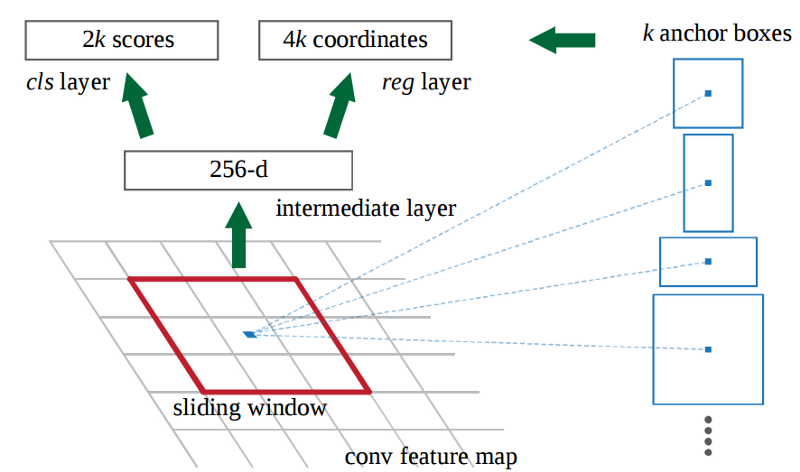
\includegraphics[scale=0.25]{faster_rcnn.png}
\caption{Region Proposal Network (RPN)}
\label{fig:fasterrcnn}
\end{center}
\end{figure}
\item \textbf{Overfeat} [22]: ganador del ILSVRC del 2013 en localización y detección de objetos, este trabajo mostró que entrenar una red convolucional para simultáneamente clasificar, localizar y detectar objetos en imágenes puede potenciar el acierto tanto en clasificación como en detección y localización. Posteriormente, ha sido reemplazado por SSD y YOLO para tareas que requieran una mejor detección en tiempo real.
\item \textbf{SSD} [23]: existen modelos más rápidos que Faster R-CNN como R-FCN que trata de mejorar la velocidad del sistema maximizando el cómputo compartido [24] o SSD. Esta última proporciona grandes ganancias en velocidad respecto a Faster R-CNN realizando las fases de generación de regiones de interés y posterior clasificación de forma conjunta (\textit{Single Shot MultiBox Detector}). Como resultado obtiene una gran cantidad de bounding box de las cuales la mayoría no son útiles. Aplicando en ellas las técnicas \textit{non-maximum suppression} y \textit{hard-negative mining} se consiguen las detecciones finales.
\item \textbf{YOLO} [25]: este sistema usa un enfoque diferente a los anteriores ya que aplica una sóla red neuronal a la imagen completa. Esta red divide la imagen en regiones y predice los bounding box y probabilidades de cada región. Posteriormente estas son ponderadas con las probabilidades para obtener las detecciones definitivas. Esto lo hace, según indican los autores, cien veces más rápido que Fast R-CNN, por ejemplo, manteniendo un acierto similar. En la última versión, YOLOv2, se introducen algunas mejoras como FCN.
\end{itemize}

\subsection{Segmentación usando redes neuronales}
%-------------------------------------------------------------------------
\bibliography{}\\
$\left[1\right]$  "Introduction to the Special Issue on Robotics and Computer Vision", J. Braz. Comp. Soc. vol. 4 no. 3 Campinas Apr. 1998\\
$\left[2\right]$  Luis Pérez, Íñigo Rodríguez, Nuria Rodríguez, Rubén Usamentiaga, and Daniel F. Gar-
cía.   "Robot  guidance  using  machine  vision  techniques  in  industrial  environments:  A comparative review". Sensors, 16(3), 2016. \\
$\left[3\right]$  Remigiusz Labudzki, Stanislaw Legutko, and Pero Raos.  "The essence and applications
of machine vision". 21:903–909, 08 2014.\\
$\left[3,1\right]$  "Computer Vision for Autonomous Vehicles: Problems, Datasets and State-of-the-Art",
Joel Janai, Fatma Güney, Aseem Behl, Andreas Geiger. Autonomous Vision Group, Max Planck Institute for Intelligent Systems, Spemannstr. 41, D-72076 T  ̈ubingen, Germany
Computer Vision and Geometry Group, ETH Z̈urich, Universit ̈atstrasse 6, CH-8092 Z  ̈urich, Switzerland. 2017.\\
$\left[4\right]$  J. McCarthy, M. L. Minsky, N. Rochester, and C. E. Shannon, “A proposal for the
dartmouth summer research project on artificial intelligence, august 31, 1955”, AI
magazine, vol. 27, no. 4, p. 12, 2006.\\
% meter referencias ia e ml
$\left[6,1\right]$  L. Deng and D. Yu, “Deep learning: Methods and applications”, Tech. Rep.,
2014. \\
$\left[6,2\right]$  "Implementation of Training Convolutional Neural Networks", Tianyi Liu, Shuangsang Fang, Yuehui Zhao, Peng Wang, Jun Zhang. University
of
Chinese
Academy
of
Sciences,
Beijing,
China, 2015.\\
$\left[6,3\right]$  Kovalev, Vassili & Kalinovsky, Alexander & Kovalev, Sergey. (2016). "Deep Learning with Theano, Torch, Caffe, TensorFlow, and Deeplearning4J: Which One Is the Best in Speed and Accuracy?"\\
$\left[6,4\right]$  "Mask R-CNN", Kaiming He, Georgia Gkioxari, Piotr Dollár, Ross Girshick. Facebook AI Research (FAIR). 2017\\
$\left[7\right]$  A. W. M. Smeulders, D. M. Chu, R. Cucchiara, S. Calderara, A. Dehghan, and
M. Shah. "Visual tracking: An experimental survey". IEEE Transactions on Pattern
Analysis and Machine Intelligence, 36(7):1442–1468, July 2014.\\
$\left[8\right]$  K. Briechle and U. D. Hanebeck, “Template matching using fast
normalized  cross  correlation,”  in Proc.  SPIE,  vol.  4387.  2001, pp. 95–102.\\
$\left[9\right]$  S. Baker and I. Matthews, “Lucas-Kanade 20 years on: A unifying framework,” IJCV, vol. 56, no. 3, pp. 221–255, 2004.\\
$\left[10\right]$  H.  T.  Nguyen  and  A.  W.  M.  Smeulders,  “Fast  occluded  object tracking by a robust appearance filter,”
IEEE Trans. Pattern Anal. Mach. Intell., vol. 26, no. 8, pp. 1099–1104, Aug. 2004.\\
$\left[11\right]$  D.  Comaniciu,  V.  Ramesh,  and  P.  Meer,  “Real-time  tracking  of non-rigid objects using mean shift,” in
Proc. IEEE CVPR, Hilton Head Island, SC, USA, 2000.\\
$\left[12\right]$  H.  T.  Nguyen  and  A.  W.  M.  Smeulders,  “Robust  track  using foreground-background  texture discrimination,” IJCV,  vol.  68, no. 3, pp. 277–294, 2006.\\
$\left[13\right]$  Z.    Kalal,    J.    Matas,    and    K.    Mikolajczyk,    “P-N    learning:
Bootstrapping  binary  classifiers  by  structural  constraints,”  in
Proc. IEEE CVPR
, San Francisco, CA, USA, 2010.\\
$\left[14\right]$  David Held, Sebastian Thrun, and Silvio Savarese. "Learning to track at 100 FPS
with deep regression networks". CoRR, abs/1604.01802, 2016.\\
$\left[15\right]$  Babenko,  B.,  Yang,  M.H.,  Belongie,  S.:  "Visual  tracking  with  online  multiple  in-
stance learning. In: Computer Vision and Pattern Recognition", 2009. CVPR 2009.
IEEE Conference on. pp. 983–990. IEEE (2009)\\
$\left[16\right]$  Tao, R., Gavves, E., Smeulders, A.W.M.: "Siamese instance search for tracking". In:
Proceedings of the IEEE Conference on Computer Vision and Pattern Recognition
(2016)\\
$\left[17\right]$  Amir Sadeghian, Alexandre Alahi, and Silvio Savarese. "Tracking the untrackable:
Learning to track multiple cues with long-term dependencies".
arXiv preprint
arXiv:1701.01909, 2017.\\
$\left[17,1\right]$  Chris Harris and Mike Stephens. "A combined corner and edge detector". In Alvey
vision conference, volume 15, pages 10–5244. Citeseer, 1988.\\
$\left[17,2\right]$  Jianbo Shi and Carlo Tomasi. "Good features to track". In Computer Vision and
Pattern Recognition, 1994. Proceedings CVPR’94., 1994 IEEE Computer Society
Conference on, pages 593–600. IEEE, 1994.\\
$\left[17,3\right]$  "Visual people tracking with deep learning
detection and feature tracking", Marcos Pieras Sagardoy, José Maria Cañas Plaza, Universidad Rey Juan Carlos, España, 2017.\\
$\left[17,4\right]$  Alex Krizhevsky, Ilya Sutskever, and Geoffrey E Hinton. "Imagenet classification with
deep convolutional neural networks". In F. Pereira, C. J. C. Burges, L. Bottou, and
K. Q. Weinberger, editors, Advances in Neural Information Processing Systems 25,
pages 1097–1105. Curran Associates, Inc., 2012.\\
$\left[17,5\right]$  "Very Deep Convolutional Networks for Large-Scale Image Recognition"
K. Simonyan, A. Zisserman. 2015.
$\left[17,6\right]$  "Xception: Deep Learning with Depthwise Separable Convolutions",
Francois Chollet
Google, Inc. 2017.\\
$\left[17,7\right]$  Kaiming He, Xiangyu Zhang, Shaoqing Ren, and Jian Sun. "Deep residual learning
for image recognition". CoRR, abs/1512.03385, 2015.\\
$\left[17,8\right]$  "Going Deeper with Convolutions", Christian Szegedy, Wei Liu, Yangqing Jia, Pierre Sermanet, Scott Reed, Dragomir Anguelov, Dumitru Erhan, Vincent Vanhoucke, Andrew Rabinovich. 2014.
$\left[17,9\right]$  "Inception-v4, Inception-ResNet and the Impact of Residual Connections on Learning",
Christian Szegedy, Sergey Ioffe, Vincent Vanhoucke, Alex Alemi. 2016.\\
$\left[18\right]$  "DSSD : Deconvolutional Single Shot Detector",
Cheng-Yang Fu, Wei Liu, Ananth Ranga, Ambrish Tyagi, Alexander C. Berg. UNC Chapel Hill,
Amazon Inc, 2017.\\
$\left[19\right]$  "Faster R-CNN: Towards Real-Time Object Detection with Region Proposal Networks",
Shaoqing Ren, Kaiming He, Ross Girshick, Jian Sun, 2016.\\
$\left[20\right]$  "Rich feature hierarchies for accurate object detection and semantic segmentation",
Ross Girshick, Jeff Donahue, Trevor Darrell, Jitendra Malik, 2013.\\
$\left[21\right]$  Ross Girshick. "Fast R-CNN". In The IEEE International Conference on Computer
Vision (ICCV), December 2015.\\
$\left[22\right]$  "OverFeat:
Integrated Recognition, Localization and Detection
using Convolutional Networks", Pierre Sermanet, David Eigen, Xiang Zhang, Michael Mathieu, Rob Fergus, Yann LeCun. Courant Institute of Mathematical Sciences, New York University. 2014.\\
$\left[23\right]$  "SSD: Single Shot MultiBox Detector".
Wei Liu, Dragomir Anguelov, Dumitru Erhan, Christian Szegedy, Scott Reed, Cheng-Yang Fu, Alexander C. Berg. 2015.\\
$\left[24\right]$  "R-FCN: Object Detection via Region-based Fully Convolutional Networks", Jifeng Dai, Yi Li, Kaiming He, Jian Sun. 2016.\\
$\left[25\right]$  "YOLO9000: Better, Faster, Stronger"
Joseph Redmon, Ali Farhadi, University of Washington, Allen Institute for AI. 2016.\\
\end{document}
